\documentclass[11pt,a4paper]{article}

\usepackage[T1]{fontenc}
\usepackage[utf8]{inputenc}
\usepackage{lmodern}
\usepackage[margin=2.4cm]{geometry}
\usepackage{microtype}
\usepackage{amsmath,amssymb}
\usepackage{booktabs}
\usepackage{tabularx}
\usepackage{multirow}
\usepackage{graphicx}
\usepackage{xcolor}
\usepackage{caption}
\usepackage{subcaption}
\usepackage{enumitem}
\usepackage{tikz}
\usetikzlibrary{positioning,arrows.meta,fit,calc,backgrounds}
\usepackage[authoryear,round]{natbib}
\usepackage[colorlinks=true,linkcolor=blue!50!black,citecolor=blue!50!black,urlcolor=blue!50!black]{hyperref}

\captionsetup{font=small,labelfont=bf}
\setlist{itemsep=2pt,topsep=4pt}
% Generated by paper/build_assets.py from committed result files. Do not edit.
\newcommand{\numBankProblems}{178}
\newcommand{\numBankTwoVar}{103}
\newcommand{\numBankThreeVar}{75}
\newcommand{\numBankStepChecked}{5,983}
\newcommand{\numBankStepUnchecked}{1,261}
\newcommand{\numBankStepFailures}{0}
\newcommand{\numPhaseOneStepChecked}{68,309}
\newcommand{\numPhaseOneStepFailures}{0}
\newcommand{\numSystemsEmitted}{164}
\newcommand{\numMethodSolutions}{811}
\newcommand{\numSkipUnparsed}{560}
\newcommand{\numSkipNoUnique}{27}
\newcommand{\numSplitTrain}{114}
\newcommand{\numSplitValid}{24}
\newcommand{\numSplitTest}{26}
\newcommand{\numTestItems}{126}
\newcommand{\numBaseGen}{0.389}
\newcommand{\numWorkedSFTGen}{0.159}
\newcommand{\numWorkedSFTLongGen}{0.183}
\newcommand{\numWorkedDPOGen}{0.000}
\newcommand{\numFormatDiffGen}{+0.071}
\newcommand{\numFormatCIGen}{[+0.02, +0.12]}
\newcommand{\numDpoWorkedDiffGen}{$-$0.159}
\newcommand{\numDpoWorkedCIGen}{[$-$0.23, $-$0.09]}
\newcommand{\numDpoTerseDiffGen}{$-$0.071}
\newcommand{\numBestMinusBaseGen}{$-$0.206}
\newcommand{\numBestMinusBaseCIGen}{[$-$0.31, $-$0.10]}
\newcommand{\numBaseMath}{0.381}
\newcommand{\numWorkedSFTMath}{0.286}
\newcommand{\numWorkedSFTLongMath}{0.389}
\newcommand{\numWorkedDPOMath}{0.111}
\newcommand{\numFormatDiffMath}{+0.071}
\newcommand{\numFormatCIMath}{[$-$0.01, +0.16]}
\newcommand{\numDpoWorkedDiffMath}{$-$0.175}
\newcommand{\numDpoWorkedCIMath}{[$-$0.30, $-$0.07]}
\newcommand{\numDpoTerseDiffMath}{$-$0.079}
\newcommand{\numBestMinusBaseMath}{+0.008}
\newcommand{\numBestMinusBaseCIMath}{[$-$0.10, +0.12]}
\newcommand{\numDpoPairs}{565}
\newcommand{\numPrefixTerse}{84.5}
\newcommand{\numPrefixWorked}{89.4}
\newcommand{\numSurfaceRuleTerse}{100}
\newcommand{\numSurfaceRuleWorked}{100}
\newcommand{\numLongerChosenTerse}{0.596}
\newcommand{\numLongerChosenWorked}{0.464}
\newcommand{\numKeywordWorstFA}{0.400}
\newcommand{\numStructWorstFA}{0.007}
\newcommand{\numStructMinRecall}{0.972}
\newcommand{\numCleanReal}{0.387}
\newcommand{\numCleanMatched}{0.398}
\newcommand{\numCleanOrig}{0.556}
\newcommand{\numSimSeed}{20270101}
\newcommand{\numSimClasses}{20}
\newcommand{\numSimLearners}{25}
\newcommand{\numSimT}{30}
\newcommand{\numBanditBestLo}{0.28}
\newcommand{\numBanditBestHi}{0.28}
\newcommand{\numDTwoHeldoutDiff}{$-$0.066}
\newcommand{\numDTwoHeldoutCI}{[$-$0.09, $-$0.04]}
\newcommand{\numSensSeed}{20271201}
\newcommand{\numSensCells}{48}
\newcommand{\numQOneBetter}{48}
\newcommand{\numQTwoBetter}{8}
\newcommand{\numQTwoSame}{28}
\newcommand{\numQTwoWorse}{12}
\newcommand{\numQThreeBetter}{8}
\newcommand{\numQThreeSame}{18}
\newcommand{\numQThreeWorse}{22}
\newcommand{\numNoRevDiff}{$-$0.043}
\newcommand{\numNoRevCI}{[$-$0.08, $-$0.01]}
\newcommand{\numSensBestLo}{0.26}
\newcommand{\numSensBestHi}{0.28}
\newcommand{\numWeakRevDiff}{+0.078}
\newcommand{\numPertLo}{+0.113}
\newcommand{\numPertHi}{+0.251}
\newcommand{\numRandRuleGridThirty}{+0.047}
\newcommand{\numRandRuleGridSixty}{+0.056}
\newcommand{\numRandRuleRepThirty}{$-$0.030}
\newcommand{\numRandRuleRepSixty}{$-$0.011}
\newcommand{\numBanditRuleRepThirty}{$-$0.011}
\newcommand{\numBanditRuleRepSixty}{+0.001}
\newcommand{\numRepRuleFixedLo}{+0.139}
\newcommand{\numRepRuleFixedHi}{+0.191}
\newcommand{\numRepChoiceLo}{+0.057}
\newcommand{\numRepChoiceHi}{+0.079}
\newcommand{\numSwitchSeed}{20280101}
\newcommand{\numSwitchSimFifteen}{$-$0.040}
\newcommand{\numSwitchSimThirty}{$-$0.041}
\newcommand{\numSwitchDiffThirty}{+0.007}
\newcommand{\numSwitchDiffSixty}{+0.023}
\newcommand{\numSwitchPassed}{failed}

% primitive input avoids "Misplaced \noalign" before \bottomrule
\makeatletter\newcommand{\tabinput}[1]{\@@input #1.tex }\makeatother

\newcommand{\eg}{e.g.,\ }
\newcommand{\ie}{i.e.,\ }

\title{\textbf{Keeping Correctness and Preference Apart in AI Mathematics Tutoring}\\[4pt]
\large Negative Results from Preference Optimisation, a Verified Tutor,\\ and a Simulation Study of When Learner Choice Can Help}
\author{Hassan Raza Shaikh\\[2pt]\small [Department, Institution]\\[2pt]\small\textit{Draft for supervisor review, November 2026}}
\date{}

\begin{document}
\maketitle

\begin{abstract}
\noindent Personalised AI tutors are often expected to learn from what learners prefer. Two
things can go wrong. The tutor's mathematics may be wrong, and what learners prefer may not
be what helps them learn. We argue that these concerns should be handled separately.
Correctness should be guaranteed by construction. Preference should only choose among
explanations that are already known to be correct, and it should itself be tested against
learning outcomes. We report three pieces of evidence for this position, on systems of
linear equations drawn from the OATutor content library.

\textbf{(1)} We fine-tuned two 1.5B-parameter models to solve a system by a \emph{requested}
method, using computer-algebra-verified multi-method solutions. Showing every arithmetic
step in the training targets helped the general model (\numFormatDiffGen{}, 95\% CI
\numFormatCIGen{}). Preference optimisation (DPO) on correct-versus-incorrect pairs lowered
accuracy in all four conditions tested, by up to \numDpoWorkedDiffMath{}. No fine-tuned
model clearly exceeded its untrained base. The DPO pairs could be told apart by a
surface rule in \numSurfaceRuleWorked\% of cases. This is consistent with a known failure
mode of DPO on low-edit-distance pairs.

\textbf{(2)} We built a tutor in which every displayed equation is checked against the true
solution (\numBankStepChecked{} equations in the problem bank and \numPhaseOneStepChecked{}
in the Phase~1 training targets, with no failures). The tutor keeps two learner signals
apart: what the learner \emph{liked} and what \emph{worked}.

\textbf{(3)} In a pre-specified simulation study, with sensitivity analysis and replication
on fresh random seeds, a mastery-based fading rule beat fixed worked examples in every
setting tested. A per-learner Thompson-sampling bandit never reliably beat the rule.
Letting learners choose their help beat the rule only when learners differed substantially
in what helped them \emph{and} their preferences tracked it strongly. Two apparent findings
from a single-seed grid failed to replicate and are retracted, and a pre-registered policy
variant failed its criteria.

Most of these results agree with earlier empirical work. Our contribution is to bring them
together into a design and a testable research question: do learners' preferences predict
what helps them? We also provide a reproducible, verified testbed and a pre-registered
classroom study design to answer it.
\end{abstract}

\vspace{0.5em}
\noindent\textbf{Keywords:} intelligent tutoring systems; learner control; preference optimisation; DPO; verified explanations; worked examples; simulation; negative results

% =====================================================================
\section{Introduction}
\label{sec:intro}

Large language models (LLMs) make it cheap to produce explanations, hints and worked
solutions for mathematics practice. They also make it cheap to produce wrong ones. In a
controlled study using OATutor problems, the help that ChatGPT produced did not pass the
authors' quality checks for about a third of the problems (32\%). Self-consistency sampling
brought this close to 0\% for algebra
\citep{pardos2024chatgpt}. A tutor that shows a wrong worked step to a novice does active
harm. A novice is the learner least able to notice the error.

A second, quieter problem concerns \emph{personalisation}. It is attractive to build tutors
that adapt to what each learner prefers, such as the kind of help they choose or the
explanations they rate highly. But learner control has not reliably improved learning. A
meta-analysis of learner control within educational technology found an overall effect that
was ``almost zero ($g = 0.05$)'' \citep{karich2014updated}. The idea that learners know best,
including the closely related learning-styles idea, is not supported by the research
reviewed by \citet{kirschner2013learners} and \citet{pashler2008learning}.

This paper starts from a project that initially merged these two concerns. Its first phase
used \emph{preference optimisation} (DPO; \citealp{rafailov2023direct}) to make small models
prefer correct solutions over incorrect ones. The preference signal there was
correctness, which a computer algebra system can already decide exactly. The results
(Section~\ref{sec:study1}) were negative. That led us to the position this paper
develops:

\begin{quote}
\emph{Keep correctness and preference apart. Guarantee correctness by construction. Let
preference choose only among explanations that are already correct. Then test whether
preference predicts learning, rather than assume it.}
\end{quote}

\paragraph{Research questions.}
\begin{enumerate}[label=\textbf{RQ\arabic*}]
  \item Can small, locally trainable LLMs be fine-tuned to solve linear systems by a
        requested method, and does preference optimisation on correctness pairs help?
  \item Can a tutor's displayed mathematics be verified step by step, so that
        personalisation never trades away correctness?
  \item Within an explicit learner model, under what conditions should a tutor (a) fade
        support by mastery, (b) learn each learner's best help from outcomes, or (c) let
        learners choose?
\end{enumerate}

\paragraph{Contributions and what is not claimed.}
\begin{itemize}
  \item \textbf{A verified multi-method solution engine and corpus.} It covers real OATutor
        systems solved by six methods. Final answers are checked by exact back-substitution,
        and every parseable displayed equation is checked at the true solution, with checks
        that are shown to catch injected errors (Section~\ref{sec:engine}). Traditional
        intelligent tutors are also correct by construction. The point here is to use that
        property as training data and as the explanation source for a tutor that
        personalises.
  \item \textbf{Negative fine-tuning results with uncertainty estimates}
        (Section~\ref{sec:study1}). These agree with DPO failure modes reported by
        \citet{pal2024smaug} and \citet{pang2024iterative}. We do not claim a new failure
        mode, and the causal test of our pair-construction hypothesis is still to be run.
  \item \textbf{A tutor design and implementation that records ``liked'' and ``worked''
        separately}, with study tooling (randomisation, counterbalanced quizzes,
        privacy-by-design logging) (Section~\ref{sec:system}).
  \item \textbf{A pre-specified simulation analysis with sensitivity and replication}
        (Section~\ref{sec:study2}). Its main results agree with real-student findings on
        adaptive fading \citep{salden2010expertise} and on population-level versus
        personalised bandit policies \citep{schmucker2025learning}. It adds a map of the
        conditions under which learner choice can pay off. The simulator's parameters are
        invented, so these results show how the mechanism behaves, not whether children
        learn more.
  \item \textbf{A methods lesson} from two single-seed findings that failed to replicate,
        and a \textbf{pre-registered classroom study design} (Section~\ref{sec:proposed}).
\end{itemize}

% =====================================================================
\section{Related work}
\label{sec:related}

\paragraph{LLM-generated help and its errors.}
\citet{pardos2023learning} compared ChatGPT-generated and human-authored algebra hints in
OATutor, and reported that 70\% of the ChatGPT hints passed manual quality checks. In a
larger study ($N = 274$), learning gains from ChatGPT help were not statistically different
from human-authored help, yet before mitigation about a third of problems (32\%) had
generated help that did not pass quality checks \citep{pardos2024chatgpt}. Classical tutors built on expert models avoid this
problem by construction, but they need hand-authored content. Our engine sits between the
two. Its content is generated, but deterministically, by a computer algebra system
\citep{meurer2017sympy}, and it is verified rather than sampled.

\paragraph{Preference optimisation on reasoning tasks.}
DPO fits a policy directly to preference pairs without a separate reward model
\citep{rafailov2023direct}. \citet{pal2024smaug} prove that minimising the usual DPO
objective may push the probability of the \emph{preferred} response down, provided the margin
between preferred and dispreferred responses grows. They also show empirically that this
happens especially when the edit distance between paired completions is low. They propose
DPO-Positive to avoid it. \citet{pang2024iterative} train on correct-versus-incorrect
chains of thought sampled from the model itself, and report that an added negative
log-likelihood term was crucial. Our Phase~1 pairs were offline, constructed rather than
sampled, and nearly identical. That puts them squarely in the regime both papers warn
about.

\paragraph{Worked examples, fading and expertise reversal.}
The expertise-reversal effect \citep{kalyuga2003expertise} is the observation that support
which helps novices can stop helping, or hinder, more advanced learners. This motivates
fading worked examples into problem solving \citep{renkl2003structuring}. In a tutored
setting, \citet{salden2010expertise} compared fixed and adaptive fading of worked examples,
with results favouring fading adapted to each learner. Our \emph{mastery rule} is a simple
version of this idea. We include it as a strong baseline, not as a contribution.

\paragraph{Learner control and learner preferences.}
Beyond the near-zero average effect in \citet{karich2014updated}, \citet{mihalca2017accuracy}
studied learner control in problem solving and reported that the accuracy of learners'
metacognitive judgements moderated how effective learner control was. Our simulation
parameter $\rho$ (how well stated preference tracks efficacy) is a simple formal stand-in for
that moderator.

\paragraph{Bandits and reinforcement learning for instruction.}
\citet{doroudi2019where} review decades of reinforcement learning for instructional
sequencing, and argue that it has worked best when constrained by learning-science theory.
At large scale, \citet{schmucker2025learning} learned which assistance action to show after
an incorrect answer, using multi-armed bandits over 43,000 actions. They found that
personalised contextual-bandit policies often produced effects ``too small'' to beat
well-optimised policies that give every student the same action. Our per-learner bandit uses
Thompson sampling \citep{thompson1933likelihood,russo2018tutorial}. We evaluate it only in
simulation. As \citet{doroudi2017robust} caution, a policy that looks good under one
simulated student model can fail under another. This is why we vary the simulator's
assumptions (Section~\ref{sec:sens}).

\paragraph{Knowledge tracing and content.}
Mastery is estimated with Bayesian Knowledge Tracing \citep{corbett1995knowledge}. Problems
come from OATutor, an open-source adaptive tutor with CC~BY-licensed content adapted from
OpenStax textbooks \citep{pardos2023oatutor}.

% =====================================================================
\section{A verified multi-method solution engine}
\label{sec:engine}

\paragraph{Source data.}
We extracted all 13,287 problems from OATutor-Content, pinned to commit \texttt{2f27a59}. Of
these, 751 are systems-of-equations problems. In OATutor, each problem is solved one way: the
way its lesson teaches. Multiple methods per problem therefore have to be generated. With the
first parser, \numSystemsEmitted{} problems state a uniquely solvable linear system with 2
or 3 variables in parseable text. A further \numSkipUnparsed{} could not be parsed, and
\numSkipNoUnique{} had no unique solution. A second parser, which also reads plain-text,
run-together and augmented-matrix statements, yields \numBankProblems{} unique systems
(\numBankTwoVar{} with two variables, \numBankThreeVar{} with three) for the tutor's problem
bank.

\paragraph{Six methods, computed and checked.}
For each system, solutions are generated by every applicable method:
\begin{itemize}
  \item for two variables only: substitution, elimination and graphing;
  \item for two or three variables: Cramer's rule, matrix inverse and Gaussian elimination.
\end{itemize}
SymPy computes every number \citep{meurer2017sympy}. Each solution is emitted in a
\emph{terse} format and a \emph{worked} format, the latter showing each arithmetic step
explicitly (for example $3(3y)-4y=5 \Rightarrow 5y=5$ instead of a direct jump). A solution
is kept only if it passes all three checks:
\begin{itemize}
  \item its final answer equals the SymPy reference solution and satisfies the original
        equations exactly;
  \item no displayed step contains an irrational rendering artefact;
  \item it passes the step-level check below.
\end{itemize}

\paragraph{Step-level check.}
Any equation derived from a linear system holds at the system's solution. So every equation
displayed in a step must hold when the true solution is substituted. For chains such as
$x = 3y = 3(1) = 3$, all parseable sides must agree. Cramer's-rule determinants are checked
against $\det(A)$ and $\det(A)\cdot v$, since $v = D_v/D$. Displays the checker cannot parse
(mostly matrices) are counted as unchecked, though their values are still computed by SymPy.
\begin{itemize}
  \item \textbf{Tutor problem bank:} \numBankStepChecked{} equations checked, \numBankStepUnchecked{}
        unchecked, \numBankStepFailures{} failures.
  \item \textbf{All four Phase~1 training datasets} (terse, worked and two synthetic sets):
        \numPhaseOneStepChecked{} equations checked, \numPhaseOneStepFailures{} failures.
\end{itemize}
The checks can fail. The test suite plants a wrong right-hand side in a step, and a wrong
determinant, and asserts that each is detected. Building the checker also exposed four bugs
in the checker itself, which were fixed before these counts were produced. Two examples: a
determinant name being parsed as a function call, and an equation such as $2x+y=1$ being
misread as revealing $y=1$.

% =====================================================================
\section{Study 1: Fine-tuning small LLMs to solve by a requested method}
\label{sec:study1}

\subsection{Setup}
The \numSystemsEmitted{} systems were split \emph{by system}, so no system appears in more
than one split. The split was \numSplitTrain{} train, \numSplitValid{} validation and
\numSplitTest{} test systems, giving \numTestItems{} test items (system $\times$ applicable
method). The prompt names the requested method. We used two 1.5B-parameter models in 4-bit
precision:
\begin{itemize}
  \item a general model, Qwen2.5-1.5B-Instruct \citep{qwen2024qwen25};
  \item a mathematics-specialised model, Qwen2.5-Math-1.5B-Instruct \citep{yang2024qwen25math}.
\end{itemize}

Training used LoRA \citep{hu2021lora} on 8 layers, on Apple-silicon hardware with the MLX
framework. SFT ran for 600 iterations (learning rate $10^{-4}$, batch size 2). DPO
(learning rate $5\times 10^{-5}$, $\beta=0.1$, 400 iterations) started from the SFT model.
The DPO pairs are the verified-correct solution against a deterministically corrupted,
verified-wrong one: a sign flip, swapped values or an off-by-one error, with the solving
steps removed. The compute-matched and synthetic-data conditions used 1500 SFT iterations.
The synthetic data had 5,624 additional examples, either from randomly generated systems or
from systems whose statistics were matched to the training split.

Outputs were generated greedily and graded exactly: the final answer must satisfy the
original equations. 95\% confidence intervals come from a cluster bootstrap that resamples
the 26 test \emph{systems} (10,000 resamples), because items from the same system are not
independent. Contrasts are paired: both conditions use the same resampled systems.

\subsection{Results}

\begin{table}[t]
\centering\small
\caption{Study~1: exact answer accuracy on the \numTestItems{} held-out test items (general model: Qwen2.5-1.5B-Instruct; math model: Qwen2.5-Math-1.5B-Instruct), with
95\% cluster-bootstrap CIs over the \numSplitTest{} test systems. Source:
\texttt{data/train/ci\_results.json}.}
\label{tab:study1}
\begin{tabular}{lcccc}
\toprule
& \multicolumn{2}{c}{General model} & \multicolumn{2}{c}{Math model}\\
\cmidrule(lr){2-3}\cmidrule(lr){4-5}
Condition & Acc. & 95\% CI & Acc. & 95\% CI \\
\midrule
\tabinput{generated/tab_study1}
\bottomrule
\end{tabular}
\end{table}

\begin{table}[t]
\centering\small
\caption{Study~1: paired contrasts (difference in accuracy) with 95\% CIs. Bold: the
interval excludes zero.}
\label{tab:study1c}
\begin{tabular}{lcccc}
\toprule
& \multicolumn{2}{c}{General} & \multicolumn{2}{c}{Math}\\
\cmidrule(lr){2-3}\cmidrule(lr){4-5}
Contrast & Diff. & 95\% CI & Diff. & 95\% CI \\
\midrule
\tabinput{generated/tab_study1_contrasts}
\bottomrule
\end{tabular}
\end{table}

\begin{figure}[t]
\centering
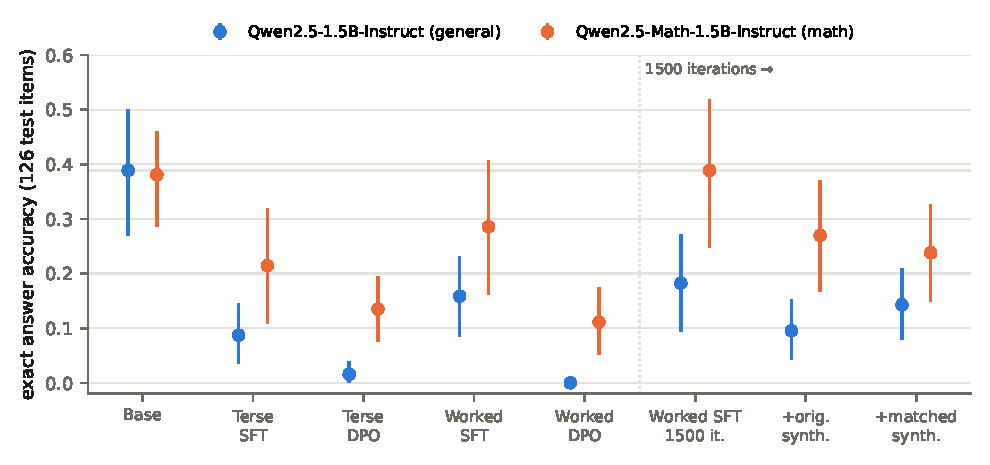
\includegraphics[width=0.95\linewidth]{generated/fig_study1.pdf}
\caption{Study~1 accuracy with 95\% CIs. The horizontal line marks the general model's base
accuracy. Conditions to the right of the dotted line use 1500 SFT iterations.}
\label{fig:study1}
\end{figure}

Tables~\ref{tab:study1} and~\ref{tab:study1c} and Figure~\ref{fig:study1} show four
results.
\begin{enumerate}
  \item \textbf{Showing the arithmetic helps, but not enough.} Worked targets beat terse ones
        for the general model (\numFormatDiffGen{}, CI \numFormatCIGen{}). The math model
        shows the same point estimate, but its interval includes zero (\numFormatCIMath{}).
        After terse SFT, outputs were perfectly formatted, yet the intermediate arithmetic was
        often invented. For example, a model correctly wrote $x=3y$ and then produced
        $15-18y=0$ where $5y=5$ was correct.
  \item \textbf{DPO hurt in every condition.} All four DPO$-$SFT contrasts are negative and
        exclude zero. The worst case is the general model with worked targets
        (\numDpoWorkedDiffGen{}), which fell to \numWorkedDPOGen{} accuracy.
  \item \textbf{No fine-tuned model clearly beat its base.} The best general SFT model is
        below its base (\numBestMinusBaseGen{}, CI \numBestMinusBaseCIGen{}). The math model
        at 1500 iterations only reaches parity (\numBestMinusBaseMath{}, CI
        \numBestMinusBaseCIMath{}).
  \item \textbf{More synthetic data did not help.} At equal compute it hurt in three of four
        cases, even when the synthetic systems' statistics were matched to the real
        training set.
\end{enumerate}

\paragraph{Why might DPO hurt? A description of the pairs.}
We measured the \numDpoPairs{} training pairs (\texttt{experiments/dpo\_pair\_diagnostics.py}).
\begin{itemize}
  \item In \numSurfaceRuleWorked\% of pairs, chosen and rejected can be separated by a surface
        rule that needs no mathematics: the rejected text always ends ``Therefore the
        solution is \ldots'', and the chosen text ends ``Solution: \ldots''.
  \item The rejected text is the chosen text's prefix plus one new line. On average it shares
        \numPrefixTerse\% (terse) and \numPrefixWorked\% (worked) of its characters with the
        start of the chosen text.
  \item By contrast, ``the longer text is chosen'' separates only \numLongerChosenTerse{}
        (terse) and \numLongerChosenWorked{} (worked) of pairs.
\end{itemize}
Pairs that differ in only a few tokens are the low-edit-distance regime in which
\citet{pal2024smaug} show DPO can lower the likelihood of the preferred response. The pairs
were also offline, not sampled from the model; \citet{pang2024iterative} use on-policy pairs
plus a likelihood term. This is a \emph{description consistent with} a known failure mode,
not a causal finding. The decisive experiment is prepared in the repository but has not been
run (it needs the original training hardware). It compares offline and on-policy,
SymPy-graded pairs at two values of $\beta$.

\paragraph{Method-faithfulness.}
The Phase~1 harness checked whether a solution used the requested method by keyword
matching. Measured on verified gold solutions, keywords wrongly accept up to
\numKeywordWorstFA{} of other methods' solutions. For example, ``Back-substitute'' in an
elimination solution counts as substitution. A structural check that inspects the
operations actually performed (Table~\ref{tab:faith} in Appendix~\ref{app:faith}) reaches
recall $\geq$ \numStructMinRecall{} and false acceptance $\leq$ \numStructWorstFA{} on the
same gold set. Its rules were refined on that set, so it still needs validating against
hand labels of real model outputs before it is used for claims.

\paragraph{Implication.}
At this scale, fine-tuning did not make the models reliable solvers, and preference
optimisation on correctness pairs made them worse. A tutor built on such a model would need
an external correctness guarantee in any case. The rest of the paper therefore takes the
correctness guarantee from the verified engine, and asks what preference \emph{should} be
used for.

% =====================================================================
\section{A tutor that keeps correctness and preference apart}
\label{sec:system}

\begin{figure}[t]
\centering
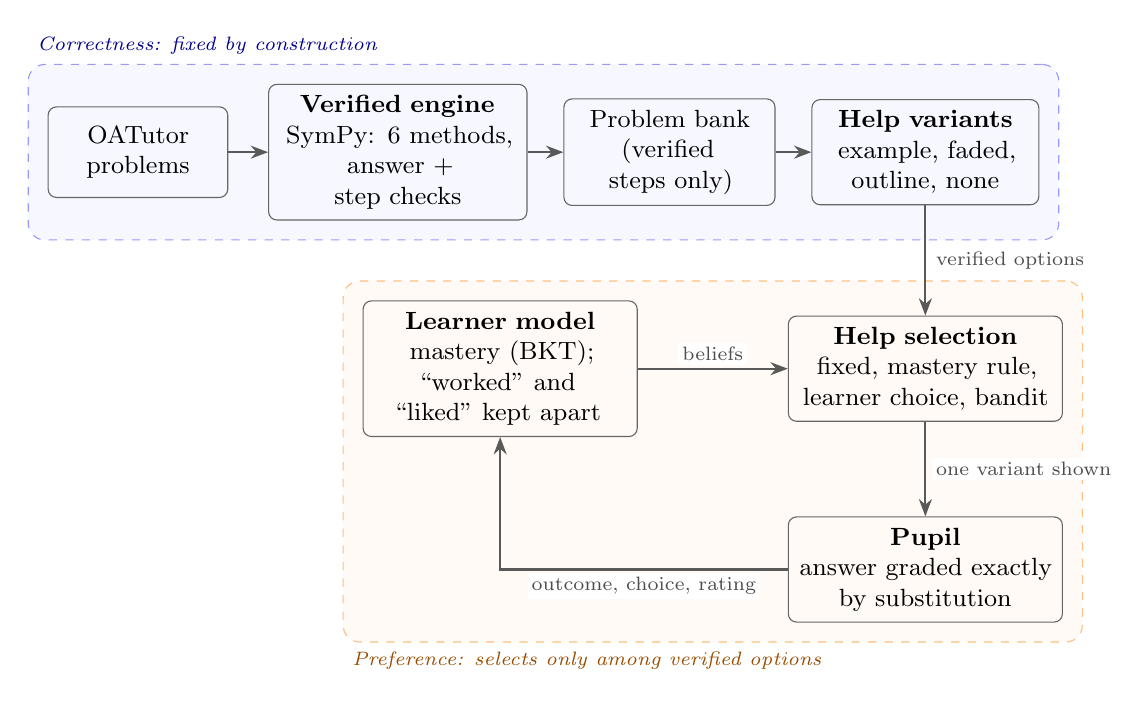
\begin{tikzpicture}[
  box/.style={draw=black!60, rounded corners=3pt, align=center, font=\small, inner sep=4pt, minimum height=1.15cm, text width=#1},
  box/.default=2.6cm,
  arr/.style={-{Stealth[length=2.2mm]}, thick, black!65},
  lab/.style={font=\scriptsize, text=black!70, fill=white, inner sep=1.5pt}]
% correctness lane
\node[box=2.0cm]  (oat)  at (0,0)    {OATutor\\problems};
\node[box=3.0cm]  (eng)  at (3.3,0)  {\textbf{Verified engine}\\SymPy: 6 methods,\\answer + step checks};
\node[box=2.4cm]  (bank) at (6.75,0) {Problem bank\\(verified steps only)};
\node[box=2.6cm]  (help) at (10.0,0) {\textbf{Help variants}\\example, faded,\\outline, none};
% preference lane
\node[box=3.2cm]  (pol)  at (10.0,-2.75) {\textbf{Help selection}\\fixed, mastery rule,\\learner choice, bandit};
\node[box=3.2cm]  (lm)   at (4.6,-2.75)  {\textbf{Learner model}\\mastery (BKT);\\``worked'' and ``liked'' kept apart};
\node[box=3.2cm]  (pup)  at (10.0,-5.3)  {\textbf{Pupil}\\answer graded exactly\\by substitution};
\draw[arr] (oat) -- (eng);
\draw[arr] (eng) -- (bank);
\draw[arr] (bank) -- (help);
\draw[arr] (help) -- node[lab, right=2pt]{verified options} (pol);
\draw[arr] (pol) -- node[lab, right=2pt]{one variant shown} (pup);
\draw[arr] (pup.west) -| node[lab, pos=0.25, below=1pt]{outcome, choice, rating} (lm.south);
\draw[arr] (lm) -- node[lab, above=1pt]{beliefs} (pol);
% lanes
\begin{scope}[on background layer]
\node[draw=blue!40, dashed, rounded corners=6pt, fill=blue!3, inner sep=7pt, fit=(oat)(eng)(bank)(help), label={[font=\scriptsize\itshape, text=blue!55!black, anchor=south west]north west:Correctness: fixed by construction}] {};
\node[draw=orange!50, dashed, rounded corners=6pt, fill=orange!4, inner sep=7pt, fit=(lm)(pol)(pup), label={[font=\scriptsize\itshape, text=orange!60!black, anchor=north west]south west:Preference: selects only among verified options}] {};
\end{scope}
\end{tikzpicture}
\caption{Architecture. Correctness is fixed upstream by the verified engine. Preference
only selects among already-verified help variants. Efficacy (``worked'') and stated
preference (``liked'') are recorded separately.}
\label{fig:arch}
\end{figure}

Figure~\ref{fig:arch} shows the design. The tutor is a small web application written with
the Python standard library and SymPy, and it runs offline.

\paragraph{Help variants.}
For a target problem and method, the tutor can show one of four kinds of help, ordered from
most to least support:
\begin{itemize}
  \item a fully worked solution of a \emph{different} but similar system (an example-problem
        pair), so the target's answer is never revealed before the pupil answers;
  \item a \emph{faded} solution of the target, cut before any step that would state a final
        value;
  \item an \emph{outline} of the method, with no numbers;
  \item \emph{no help}.
\end{itemize}
After the pupil answers, the full verified solution is shown. Answers are graded exactly by
substitution into the original equations, and short diagnoses are given, such as a sign
error or swapped values.

\paragraph{Two signals, kept apart.}
For each learner and mastery band (low, mid or high BKT estimate), the tutor keeps two Beta
posteriors per help type:
\begin{itemize}
  \item \emph{efficacy}: did the learner solve the problem after this help?
  \item \emph{liking}: did they choose it or rate it useful?
\end{itemize}
A teacher-set weight $w$ combines the two when the tutor chooses help:
$\text{score} = (1-w)\,\text{efficacy} + w\,\text{liking}$. Recording both lets a study ask
whether they agree, instead of assuming they do.

\paragraph{Modes and study tooling.}
The tutor has four modes for choosing help:
\begin{itemize}
  \item \emph{fixed}: always the same help, the control condition;
  \item \emph{mastery rule}: worked example, then faded, then outline as BKT mastery rises;
  \item \emph{learner choice}: the pupil picks from two offered help types;
  \item \emph{bandit}: Thompson sampling over help types, pooled with class-level evidence.
\end{itemize}
For classroom studies it supports block randomisation of pupils to conditions,
counterbalanced parallel pre- and post-test forms built from held-out problems, a
teacher page protected by a key, and a learner-code allow-list. Logging is privacy-preserving
by design: it stores pseudonymous codes and the \emph{parsed numbers} of an answer, never
the raw typed text. The repository's test suite (47 tests) includes deliberately injected
faults for each safeguard.

% =====================================================================
\section{Study 2: Simulating help-selection policies}
\label{sec:study2}

\subsection{Simulated learners}
We cannot test learning effects without learners. We use simulation only to examine how the
policies \emph{behave} under explicit, varied assumptions. Each simulated learner has the
following hidden properties, invisible to the tutor:
\begin{itemize}
  \item \textbf{Skill levels.} A level in \{0 novice, 1 partial, 2 mastered\} for each of
        three skills (methods), drawn initially with probabilities 0.6, 0.3 and 0.1.
  \item \textbf{Learning.} After help of type $a$, the learner moves up one level with
        probability $\min(0.95, B[\ell][a]\cdot m_a)$. The base table $B$
        (Appendix~\ref{app:sim}) encodes expertise reversal \citep{kalyuga2003expertise}:
        worked examples help novices most, and lighter help helps partial learners more.
        The factor $m_a = \exp(\sigma z_a)$, with $z_a \sim N(0,1)$, is the learner's
        individual multiplier. $\sigma$ controls how much learners differ in what helps
        them.
  \item \textbf{Answering.} The learner answers correctly with probability 0.10, 0.50 or
        0.92 by level.
  \item \textbf{Stated liking.} The learner's liking for help type $a$ is
        $\rho z_a + \sqrt{1-\rho^2}\,\epsilon_a$. So $\rho$ sets how well stated preference
        tracks what actually helps; $\rho \approx 0$ corresponds to poor metacognitive
        accuracy \citep{mihalca2017accuracy}.
\end{itemize}
Every policy uses the \emph{same} BKT pacing code as the real tutor, with OATutor's default
parameters, and the same Beta-posterior code. Only the choice of help differs. Each run
simulates classes of 25 learners whose turns are interleaved, so that class-level pooling
behaves as it would in a classroom. Contrasts are paired by class, and 95\% CIs come from a
bootstrap over classes. The primary outcome is the share of the three skills a learner has
\emph{truly} mastered (hidden level 2) after $T$ problems.

\subsection{Protocol: development seed, held-out seed, fresh seed}
Six variants of the bandit were compared on a \emph{development} seed: different reward
definitions, prior strengths and pooling weights. The best-looking variant (a soft prior
favouring the mastery rule) was then evaluated once on a \emph{held-out} seed. It did
\emph{not} replicate. On the held-out seed it was worse than the mastery rule when learners
do not differ (\numDTwoHeldoutDiff{}, CI \numDTwoHeldoutCI{}), so the original design was
kept. All results below use the original bandit design.

\subsection{Main results (held-out seed)}

\begin{table}[t]
\centering\small
\caption{Study~2, held-out seed \numSimSeed{} (\numSimClasses{} classes $\times$
\numSimLearners{} simulated learners, $T=\numSimT$ problems each): share of skills truly
mastered, with 95\% CIs. Scenario A: $\sigma=0$. B: $\sigma=0.6$, $\rho=0.8$. C:
$\sigma=0.6$, $\rho=0$. Last column: share of choices that matched the learner's truly best
help type (scenario B). Source: \texttt{tutor/results/sim\_results\_D0\_heldout.json}.}
\label{tab:sim}
\resizebox{\linewidth}{!}{%
\begin{tabular}{lcccc}
\toprule
Policy & A: no differences & B: honest preferences & C: misleading preferences & Picks best help (B)\\
\midrule
\tabinput{generated/tab_sim_heldout}
\bottomrule
\end{tabular}}
\end{table}

\begin{table}[t]
\centering\small
\caption{Study~2, held-out seed: paired contrasts, with 95\% CIs over classes. Bold: the
interval excludes zero.}
\label{tab:simc}
\resizebox{\linewidth}{!}{%
\begin{tabular}{lccc}
\toprule
Contrast & A: no differences & B: honest preferences & C: misleading preferences\\
\midrule
\tabinput{generated/tab_sim_contrasts}
\bottomrule
\end{tabular}}
\end{table}

\begin{figure}[t]
\centering
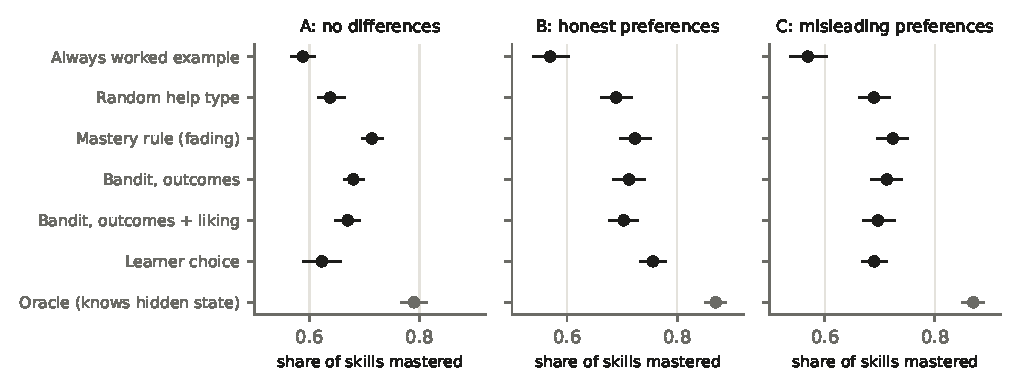
\includegraphics[width=\linewidth]{generated/fig_sim_heldout.pdf}
\caption{Study~2 on the held-out seed: share of skills truly mastered after 30 problems, with
95\% CIs over 20 classes. The oracle (grey) knows each learner's hidden state.}
\label{fig:sim}
\end{figure}

Tables~\ref{tab:sim} and~\ref{tab:simc} and Figure~\ref{fig:sim} show three results.
\begin{enumerate}
  \item \textbf{Fading by mastery beats fixed worked examples} in all three scenarios.
        That is the direction \citet{salden2010expertise} reported for adaptive fading with
        real learners. Here it largely follows from the expertise-reversal assumption built
        into the simulator; Section~\ref{sec:sens} tests what happens without it.
  \item \textbf{The bandit does not personalise.} It picks the learner's truly best help in
        \numBanditBestLo{} of decisions in every scenario, against 0.25 by chance, and it
        never beats the rule. This agrees with \citet{schmucker2025learning}, who found with
        real students that personalised policies often could not beat well-optimised
        population policies. The likely reason is the weak signal: within 30 problems,
        correctness mostly reflects what the learner already knew, not which help they just
        received.
  \item \textbf{Learner choice depends on whether preferences are honest.} It beats the
        rule only in scenario B, and it is worse when learners do not differ (scenario A).
\end{enumerate}

\subsection{Sensitivity analysis and replication}
\label{sec:sens}
To test whether these conclusions are artefacts of our chosen parameters, we ran a
pre-specified grid on a new seed (\numSensSeed). The questions and the expected outcomes were
written into the analysis code before it was run. The grid had \numSensCells{} cells:
$\sigma \in \{0, 0.3, 0.6, 1.0\}$, $\rho \in \{-0.5, 0, 0.5, 0.9\}$ and
$T \in \{15, 30, 60\}$. We also tried eight alternative learning tables: the default, a
weak-reversal table, a no-reversal table, and five random log-normal perturbations of $B$.

\paragraph{A check that could fail.}
If worked examples are best at \emph{every} level (no expertise reversal), the mastery rule
should lose to always showing worked examples. It does: \numNoRevDiff{}, CI \numNoRevCI{}. So
the simulator does not guarantee that the rule wins. The rule's advantage rests on expertise
reversal being real. With reversal present, the rule beat fixed worked examples in all
\numQOneBetter{} grid cells, in the weak-reversal table (\numWeakRevDiff{}), and in all five
perturbed tables (\numPertLo{} to \numPertHi{}).

\paragraph{Learner choice.}
Figure~\ref{fig:sens} shows learner choice minus the rule across the grid. Learner choice was
better in \numQThreeBetter{} cells, no different in \numQThreeSame{} and worse in
\numQThreeWorse{}. The gains are confined to the corner where learners differ substantially
\emph{and} their preferences track what helps.

\begin{figure}[t]
\centering
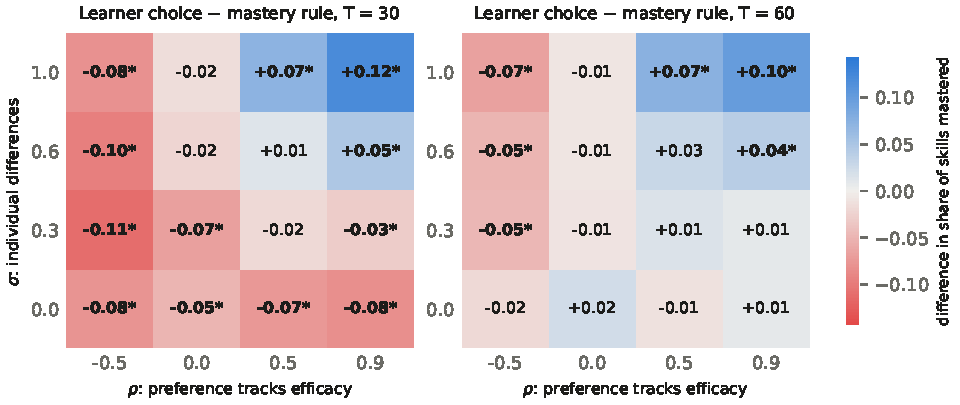
\includegraphics[width=0.92\linewidth]{generated/fig_sensitivity.pdf}
\caption{Sensitivity grid (seed \numSensSeed): learner choice minus mastery rule, in share of
skills mastered. Blue: learner choice better; red: worse; $^*$/bold: 95\% CI excludes zero.
Rows: individual differences $\sigma$. Columns: preference--efficacy match $\rho$. All cells
share one draw of simulated classes; see Table~\ref{tab:rep} for replication on new classes.}
\label{fig:sens}
\end{figure}

\paragraph{Replication on a fresh seed, and two retractions.}
On the grid seed, the bandit appeared to beat the rule in \numQTwoBetter{} cells, all at
$\sigma = 1.0$ with $T \geq 30$. An exploratory follow-up, added after seeing that result,
found that \emph{random} help beat the rule there too (\numRandRuleGridThirty{} and
\numRandRuleGridSixty{}). That suggested the bandit was winning by variety rather than by
personalising.

Every cell of a single-seed grid reuses the same simulated classes, however. Those 8
``wins'' were therefore one draw of classes, viewed across four values of $\rho$ (which the
bandit ignores) and two horizons. We re-ran twelve key cells with new classes (seed
\numSwitchSeed; Table~\ref{tab:rep}):
\begin{itemize}
  \item the bandit's gains at $\sigma = 1.0$ disappeared (\numBanditRuleRepThirty{} and
        \numBanditRuleRepSixty{}, not significant);
  \item random help no longer beat the rule (\numRandRuleRepThirty{} and
        \numRandRuleRepSixty{}, not significant).
\end{itemize}
Both claims are retracted. The robust findings replicated:
\begin{itemize}
  \item the rule beat fixed worked examples in all 12 cells (\numRepRuleFixedLo{} to
        \numRepRuleFixedHi{});
  \item learner choice beat the rule in all four cells with $\sigma \geq 0.6$ and
        $\rho = 0.9$ (\numRepChoiceLo{} to \numRepChoiceHi{});
  \item learner choice was worse in all four cells with $\rho = -0.5$.
\end{itemize}
At $\sigma = 1.0$ and $\rho = 0.5$, the gain from learner choice was not robust.

\begin{table}[t]
\centering\small
\caption{Replication on fresh seed \numSwitchSeed{}: paired contrasts in share of skills
mastered. $^{+}$/$^{-}$: 95\% CI above or below zero. Source:
\texttt{tutor/results/sensitivity.json} (\texttt{replication\_fresh\_seed}).}
\label{tab:rep}
\begin{tabular}{cccrrrr}
\toprule
$\sigma$ & $\rho$ & $T$ & Rule $-$ fixed & Bandit $-$ rule & Random $-$ rule & Choice $-$ rule\\
\midrule
\tabinput{generated/tab_replication}
\bottomrule
\end{tabular}
\end{table}

\paragraph{A pre-registered variant that failed.}
The retracted ``variety'' result had suggested a hybrid policy: follow the rule, but switch
to the next-nearest help type after each wrong answer. We tested it with success criteria
fixed in advance (\texttt{tutor/switch\_rule.py}, seed \numSwitchSeed):
\begin{itemize}
  \item[(a)] no significant loss against the rule when learners are similar;
  \item[(b)] a significant gain at $\sigma = 1.0$ with $T \geq 30$.
\end{itemize}
It \textbf{\numSwitchPassed} both. It lost when learners do not differ (\numSwitchSimFifteen{}
and \numSwitchSimThirty{} at $T = 15$ and 30, both significant), and its gains at
$\sigma = 1.0$ were not significant (\numSwitchDiffThirty{} and \numSwitchDiffSixty{}). It
was not added to the tutor.

% =====================================================================
\section{Proposed classroom study}
\label{sec:proposed}
The simulations narrow the open question to two quantities that only real learners can
reveal: how much learners differ in which help works for them, and whether their stated
preferences track it. We therefore propose, as a pre-registered study, randomising pupils
within classes to three arms: fixed worked examples, the mastery rule, and learner choice.
Learning is measured by counterbalanced, parallel pre- and post-tests built from held-out
problems.
\begin{itemize}
  \item \textbf{RQ-A:} rule versus fixed.
  \item \textbf{RQ-B:} learner choice versus rule.
  \item \textbf{RQ-C} (central): for each pupil, does the help they ``liked most'' coincide
        with the help after which they ``worked best''?
\end{itemize}

Detecting a medium effect ($d = 0.4$) between two arms with 80\% power at $\alpha = .05$
needs about 99 pupils per arm, or about 74 per arm with pre-test adjustment, assuming a
pre/post correlation of 0.5. A first pilot of 60--90 pupils is therefore for feasibility and
effect-size estimation only. The study requires ethics approval, parental consent and pupil
assent. Draft materials are in the repository (\texttt{docs/pilot/}).

% =====================================================================
\section{Discussion}
\label{sec:discussion}

\paragraph{What is new, and what is not.}
Most individual results here agree with prior work:
\begin{itemize}
  \item the DPO failure, with \citet{pal2024smaug} and \citet{pang2024iterative};
  \item the bandit result, with real-student evidence from \citet{schmucker2025learning};
  \item fading by mastery, with \citet{salden2010expertise};
  \item the conditional value of learner choice, with \citet{mihalca2017accuracy} and the
        near-zero average effect in \citet{karich2014updated}.
\end{itemize}
What this paper adds is the combination:
\begin{itemize}
  \item a design that separates correctness (verified upstream) from preference (selection
        among correct options) and records ``liked'' and ``worked'' as distinct signals;
  \item a verified multi-method corpus from real tutoring content;
  \item a simulation that maps \emph{where} learner choice can pay off, with sensitivity
        analysis and replication;
  \item a concrete, pre-registered question for a classroom study.
\end{itemize}
Our literature search (Appendix~\ref{app:search}) did not surface work on fine-tuning LLMs
to solve linear systems by a requested method, or a tutor design that keeps these two
signals apart. The search was not systematic, though, and several major indexes were not
searched, so we make no priority claim.

\paragraph{A methods lesson.}
A grid of simulation results computed from one random seed shows one draw of simulated
classes many times. Two of our grid findings (the bandit's gains and the benefit of
variety) vanished with new classes, and a policy built on one of them failed its
pre-registered test. Simulation-based claims in education are cheap to produce in large
numbers. We suggest they should routinely be replicated with independent draws, and
include a check that is able to fail, before they inform design.

\paragraph{Limitations.}
\begin{itemize}
  \item \textbf{Study~1:}
    \begin{itemize}
      \item small (1.5B, 4-bit) models;
      \item one training run per condition;
      \item only 26 test systems, so intervals are about $\pm 0.1$;
      \item one topic;
      \item the causal test of the DPO hypothesis has not been run.
    \end{itemize}
  \item \textbf{Method-faithfulness:} the structural check is validated only on gold
        solutions.
  \item \textbf{Study~2:}
    \begin{itemize}
      \item the learner model is invented and qualitative;
      \item BKT uses placeholder parameters;
      \item the results show how the mechanism behaves, not learning effects.
    \end{itemize}
  \item \textbf{The tutor:} it has not yet been used by real pupils.
\end{itemize}

% =====================================================================
\section{Conclusion}
Treating correctness as a preference to be learned did not work for small models here, and a
computer algebra system can guarantee correctness instead. Preference is better used to
choose among verified explanations. Even then, a learner's stated preference is only worth
following if it tracks what actually helps that learner. In our simulations, this held only
when learners differed substantially in what helped them and judged it accurately. Whether
real pupils meet those conditions is an empirical question. The verified tutor and study
design presented here are built to answer it.

% =====================================================================
\section*{Reproducibility}
All code, data manifests, result files and this paper's source are in the project
repository.\footnote{\url{https://github.com/Hassan-Raza-Shaikh/Preference-Learning-in-Education}}
Every number in this paper's tables and macros is generated from committed result files by
\texttt{paper/build\_assets.py}. The source data is pinned to OATutor-Content commit
\texttt{2f27a59}. Seeds are fixed throughout: the split (20260909), the CI bootstrap
(20261009), the simulation development, held-out, sensitivity and fresh seeds (20261103,
20270101, 20271201 and 20280101). The 47 automated tests run in continuous integration. The
Study~1 training runs require Apple-silicon hardware, and their generations are not
committed. The pending Study~1 experiments are scripted in \texttt{experiments/onpolicy\_dpo.py}.

\section*{Use of AI tools}
Claude Code, an AI coding assistant made by Anthropic, was used throughout this project. It
wrote and ran most of the code (data pipeline, experiments, tutor, simulations and tests),
carried out the literature search reported in Appendix~\ref{app:search}, and drafted this
manuscript, all under the author's direction. The author is responsible for the content.
No human outside the project has reviewed this work. The checks described here are
automated tests and AI-run analyses, not external review.

\section*{Ethics}
No human participants were involved in the work reported here. The proposed classroom study
will require institutional ethics approval and consent before any data collection.

\bibliographystyle{plainnat}
\bibliography{refs}

% =====================================================================
\appendix
\section{Base-model accuracy by method}
\label{app:base}
\begin{table}[h]
\centering\small
\caption{Untrained base-model accuracy by requested method on the Study~1 test set. Source:
\texttt{data/train/eval\_*\_base.json}.}
\begin{tabular}{lccc}
\toprule
Method & Test items & General & Math\\
\midrule
\tabinput{generated/tab_base_methods}
\bottomrule
\end{tabular}
\end{table}

\section{Method-faithfulness: keyword vs structural check}
\label{app:faith}
\begin{table}[h]
\centering\small
\caption{Recall (the correct method's gold solution is accepted) and false acceptance (other
methods' gold solutions are accepted) on verified gold solutions. Source:
\texttt{data/train\_worked/faithfulness\_validation.json}.}
\label{tab:faith}
\begin{tabular}{lccccc}
\toprule
& & \multicolumn{2}{c}{Keyword (Phase 1)} & \multicolumn{2}{c}{Structural}\\
\cmidrule(lr){3-4}\cmidrule(lr){5-6}
Method & Gold & Recall & False acc. & Recall & False acc.\\
\midrule
\tabinput{generated/tab_faithfulness}
\bottomrule
\end{tabular}
\end{table}

\section{Simulator parameters}
\label{app:sim}
\begin{itemize}
  \item \textbf{Base learning probabilities $B[\ell][a]$:}
    \begin{itemize}
      \item novice ($\ell=0$): example 0.30, faded 0.18, outline 0.08, none 0.04;
      \item partial ($\ell=1$): example 0.12, faded 0.25, outline 0.22, none 0.15.
    \end{itemize}
  \item \textbf{Correctness by level:} 0.10, 0.50, 0.92.
  \item \textbf{BKT parameters} (OATutor defaults): $p_{\text{init}}=p_{\text{transit}}=p_{\text{slip}}=p_{\text{guess}}=0.1$;
        mastery threshold 0.95.
  \item \textbf{Mastery bands:} low below 0.4, mid 0.4--0.8, high above 0.8. The mastery rule
        assigns example, faded and outline respectively.
  \item \textbf{Bandit:} Beta(1,1) priors plus class evidence weighted by 0.2. Preference
        weight $w = 0.3$ for the variants that use liking, and 0 otherwise.
  \item \textbf{Learner choice:} the two help types with the highest Thompson samples are
        offered; the learner picks the one with the higher liking, plus $N(0, 0.5^2)$ noise.
\end{itemize}
These values were chosen to encode the expertise-reversal effect qualitatively. They were
not fitted to data.

\section{Literature search}
\label{app:search}
On 2026-11-27, twenty web-search queries were run, and the cited sources' bibliographic
records were checked against Crossref or arXiv. Abstracts were read for: Pardos and
Bhandari (2023, 2024), Karich et al., Schmucker et al., Pal et al., Pang et al., the DPO,
LoRA and Qwen reports, Russo et al., SymPy, and (in part) Pashler et al.

For Salden et al., Doroudi et al. (2017, 2019), Mihalca et al. and Kirschner and van
Merriënboer, only bibliographic records and search-engine summaries were available: their
publisher pages returned bot challenges. They are cited here only for their general
findings. Google Scholar, ERIC, the ACM Digital Library, IEEE Xplore and conference indexes
were not searched.

The full log, with every query, is in \texttt{paper/LITERATURE\_LOG.md}.

\end{document}
